\begin{tikzpicture}[
start chain=going right,
diagram item/.style={
	minimum width=30pt,
	on chain
%	join
},
connection/.style={
%	->,
	thick,
	shorten <=2pt,
	shorten >=2pt,
}]

\newcounter{TurbnieCounter}

\newcommand\millFigure{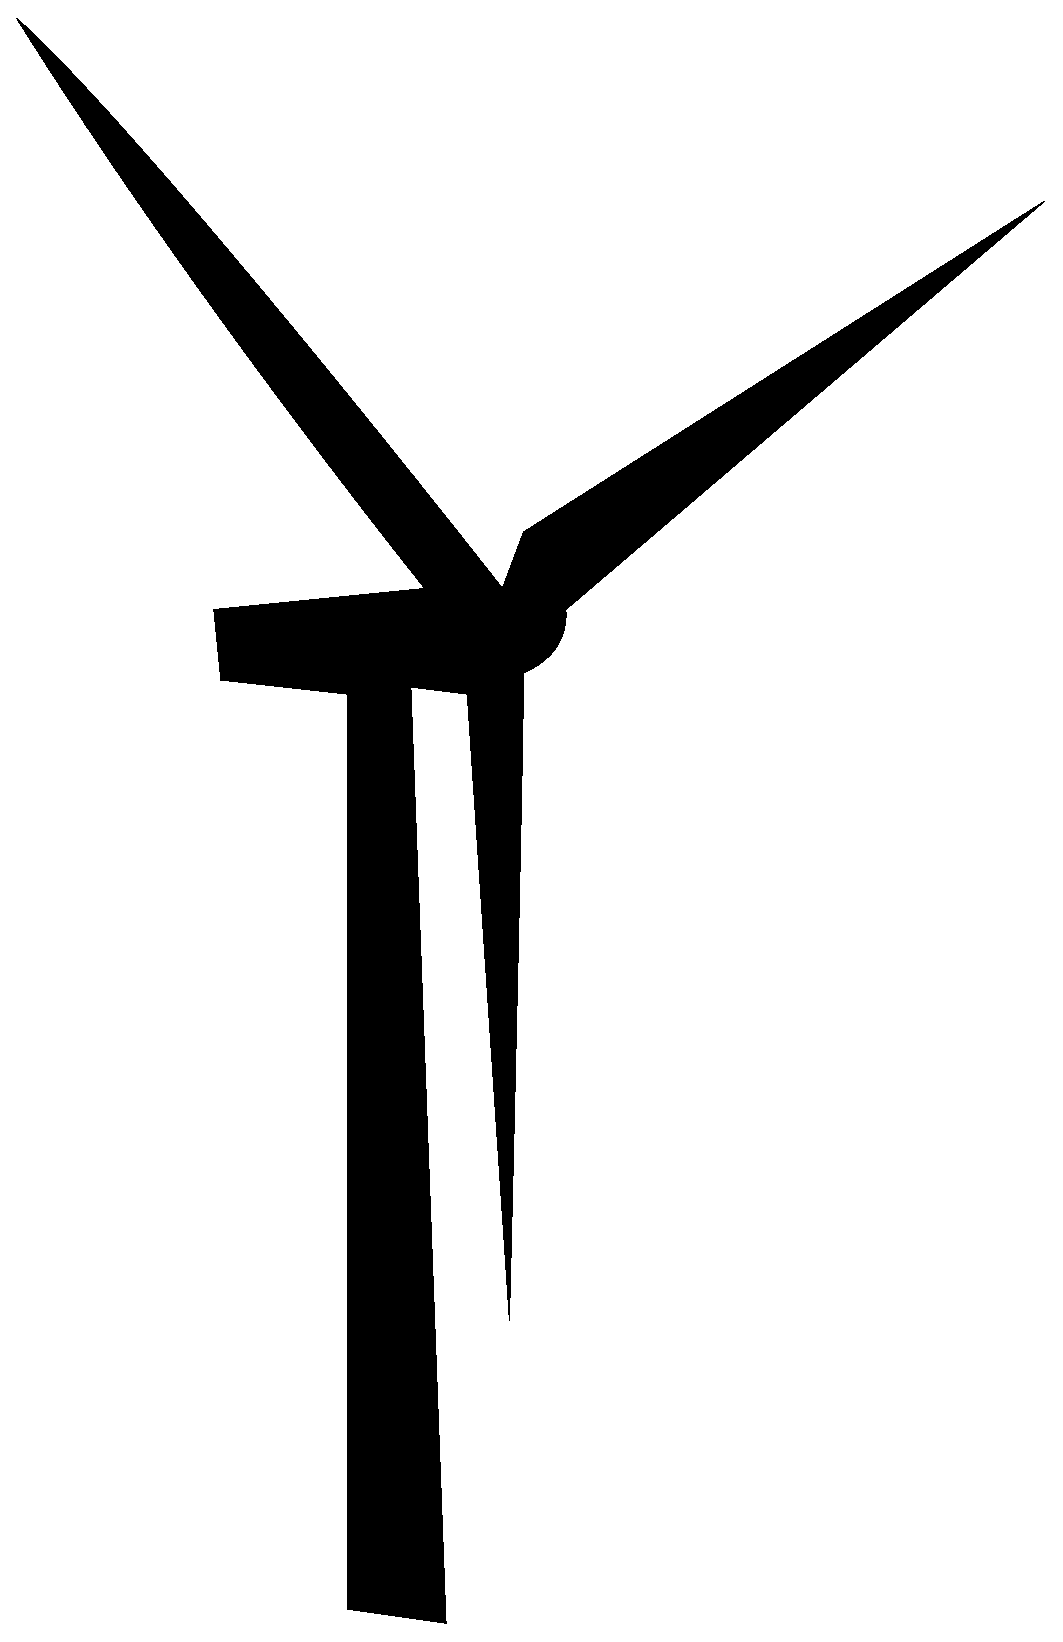
\includegraphics[width=0.5cm]{MillSiluet}}


\newcommand{\printTurbineID}{\ifnum\value{TurbnieCounter}<10 0\fi\arabic{TurbnieCounter}}
\stepcounter{TurbnieCounter}

\node [
diagram item,
label={[align=center]above:T\printTurbineID\\Load\\Balancer\\(Active)}
] (CenterNode) {\millFigure};
\stepcounter{TurbnieCounter}

\node [
draw,
below =2cm of CenterNode,
inner sep=0.5cm
] (Switch) {switch};
\draw[connection] (Switch) -- (CenterNode);


\node [
continue chain = going right,
diagram item,
label={[align=center]above:T\printTurbineID\\Database\\Shard}
] (Turbine) {\millFigure};
\stepcounter{TurbnieCounter}
\draw[connection] (Switch) -- (Turbine);

\node [
continue chain = going right,
diagram item,
label={[align=left]right:T\printTurbineID\\External\\Interface}
] (Turbine) {\millFigure};
\stepcounter{TurbnieCounter}
\draw[connection] (Switch) -- (Turbine);

\node [
continue chain = going below,
diagram item,
label={[align=left]right:T\printTurbineID\\Database\\Shard}
] (Turbine) {\millFigure};
\stepcounter{TurbnieCounter}
\draw[connection] (Switch) -- (Turbine);

\node [
continue chain = going below,
diagram item,
label={[align=left]right:T\printTurbineID\\External\\Interface}
] (Turbine) {\millFigure};
\stepcounter{TurbnieCounter}
\draw[connection] (Switch) -- (Turbine);

\node [
continue chain = going below,
diagram item,
label={[align=left]right:T\printTurbineID\\Load Balancer\\(Backup)}
] (Turbine) {\millFigure};
\stepcounter{TurbnieCounter}
\draw[connection] (Switch) -- (Turbine);

\node [
continue chain = going left,
diagram item,
label={[align=center]below:T\printTurbineID\\Database\\Shard}
] (Turbine) {\millFigure};
\stepcounter{TurbnieCounter}
\draw[connection] (Switch) -- (Turbine);

\node [
continue chain = going left,
diagram item,
label={[align=center]below:T\printTurbineID\\External\\Interface}
] (Turbine) {\millFigure};
\stepcounter{TurbnieCounter}
\draw[connection] (Switch) -- (Turbine);

\node [
continue chain = going left,
diagram item,
label={[align=center]below:T\printTurbineID\\Database\\Shard}
] (Turbine) {\millFigure};
\stepcounter{TurbnieCounter}
\draw[connection] (Switch) -- (Turbine);

\node [
continue chain = going left,
diagram item,
label={[align=right]left:T\printTurbineID\\Load Balancer\\(Backup)}
] (Turbine) {\millFigure};
\stepcounter{TurbnieCounter}
\draw[connection] (Switch) -- (Turbine);

\node [
continue chain = going above,
diagram item,
label={[align=right]left:T\printTurbineID\\Database\\Shard}
] (Turbine) {\millFigure};
\stepcounter{TurbnieCounter}
\draw[connection] (Switch) -- (Turbine);

\node [
continue chain = going above,
diagram item,
label={[align=right]left:T\printTurbineID\\External\\Interface}
] (Turbine) {\millFigure};
\stepcounter{TurbnieCounter}
\draw[connection] (Switch) -- (Turbine);

\node [
continue chain = going above,
diagram item,
label={[align=right]left:T\printTurbineID\\Database\\Shard}
] (Turbine) {\millFigure};
\stepcounter{TurbnieCounter}
\draw[connection] (Switch) -- (Turbine);

\node [
continue chain = going right,
diagram item,
label={[align=center]above:T\printTurbineID\\External\\Interface}
] (Turbine) {\millFigure};
\stepcounter{TurbnieCounter}
\draw[connection] (Switch) -- (Turbine);



%\node [
%continue chain = going below,
%diagram item,	
%label={[align=center]right:T04\\LoadBalancer\\Primary}
%] (end1) {\millFigure};

%\draw (endBranch1) -> (end1) node{};
%\draw (endBranch1) -> (startBranch) node{};
%\draw (endBranch1) -> (start) node{};
%\draw (end1) -> (startBranch) node{};



%\draw (endBranch2) -> (end2) node{};

\end{tikzpicture}